 \documentclass{beamer}
\beamertemplatenavigationsymbolsempty
\usepackage{amsmath, amssymb, hyperref, graphics, tikz}
\usepackage[normalem]{ulem} %for strikeout \sout{ }

\usepackage{tikzsymbols} %for smileys

\newcommand{\C}{\mathbb{C}}
\newcommand{\Z}{\mathbb{Z}}
\newcommand{\R}{\mathbb{R}}
\newcommand{\N}{\mathbb{N}}
\DeclareMathOperator{\Real}{Re}
\DeclareMathOperator{\Imag}{Im}
\begin{document}
\begin{frame}{Section 9: Cauchy's Integral Formula and Consequences}
\begin{theorem}[Cauchy's integral formula] Let $\gamma$ be a simple contour described in the positive direction.  Let $w$ lie inside $\gamma$.  Suppose that $f$ is analytic on a simply connected region $D$ containing $\gamma$ and its interior.  Then:

$$f(w)=\frac{1}{2\pi i} \int_\gamma\frac{f(z)}{z-w}dz.$$

\end{theorem}
\begin{block}{Uses of Cauchy's Integral Formula}
\begin{itemize}
    \item Calculate contour integrals
    \item Values of $f$ inside a contour determined by values on boundary
    \item \alert{Proving $f$ has convergent Taylor series!}
\end{itemize}
\end{block}

\end{frame}


\begin{frame}{High level overview of Cauchy's Integral Formula}

Many proofs we see have essential no real ideas to them -- they're just unpacking definitions.  Cauchy's integral formula has one real idea (Point 1) and one sneaky trick (Point 2).

    
\begin{block}{Sketch of proof}
\begin{enumerate}
    \item Theorem 9.1 ``Deforming contours'': replace $\gamma$ with $w+\varepsilon e^{2\pi i t}$ and take $\varepsilon\to 0$
    \item  $$????\quad\frac{f(z)-f(w)}{z-w}\quad????$$
    \item \sout{Profit} Prove the Theorem
\end{enumerate}
\end{block}
Theorem 9.1 depends on Cauchy's Theorem, and it and the ideas that go into it are independently useful.


\end{frame}
\begin{frame}{Theorem 9.1 Deforming Contours}
\begin{theorem} Let $\gamma$ be a simple contour described in the positive direction.  Let $z_0$ be a point inside $\gamma$, and let $C$ be another simple contour in positive direction, contained entirely inside $\gamma$. Suppose that $f$ is analytic on a region $D$ which contains $\gamma, C$ and all points in between.  Then
$$\int_\gamma f(z)dz=\int_C f(z)dz$$
\end{theorem}
\begin{itemize}
    \item Crucially, $D$ need not be simply connected
    \item Proof: join $C$ and $\gamma$ together by two paths, and rearrange contours to apply Cauchy.
\end{itemize}

\end{frame}

\begin{frame}{Proving Cauchy's Integral Formula}
Let $C_\varepsilon(w)$ be the circle of radius $\varepsilon$ around $w$.  
By Deforming Contours, we have
$$\int_\gamma \frac{f(z)}{z-w}dz=\int_{C_\varepsilon(w)} \frac{f(z)}{z-w}dz$$
Using the trick, we have that this is
$$=\int_{C_\varepsilon(w)}  \frac{f(z)-f(w)}{z-w}dz+\int_{C_\varepsilon(w)} \frac{f(w)}{z-w}dz$$
We already computed that the second integral is $2\pi i f(w)$, so we need to see the first integral tends toward zero.
\end{frame}

\begin{frame}{Vanishing of the first integral}
\begin{block}{We use the ML estimate}
\begin{itemize}
    \item As $\varepsilon\to 0$, $z\to w$, and the integrand $\frac{f(z)-f(w)}{z-w}\to f^\prime(w)$
    \item In particular, integrand is bounded by some $M$.
 \item The length of $C_{\varepsilon}(w)=2\pi \varepsilon$.
\end{itemize}
Thus
$$\left|\int_{C_\varepsilon(w)}  \frac{f(z)-f(w)}{z-w}dz\right|\leq M2\pi\varepsilon$$
And so the integral $\to 0$ as $\varepsilon\to 0$


\end{block}
\end{frame}
\begin{frame}{Contour integrals via of Cauchy's Integral Formula}
\begin{example}[Section 9.3]Let $\gamma$ be the simple, positively oriented triangular contour from 0 to $2-3i$ to $2+2i$ and back to zero.  Evaluate
$$\int_\gamma \frac{e^z}{z-1}dz \quad \int_\gamma \frac{e^z}{z+1}dz \quad \int_\gamma \frac{1}{z^2-1}dz $$
$$\int_\gamma \frac{ze^{z^2}}{(z-1)(2z-1)}dz \quad \int_\gamma \frac{e^{z^2}}{z^2-1}dz$$

\end{example}

\begin{block}{Tips and Tricks}
\begin{itemize}

\item \alert{Draw Picture} containing contour and "bad" points
\item Avoid partial fractions -- deform contour instead \Cooley
\end{itemize}
\end{block}
\end{frame}

\begin{frame}{I had to use this one at some point, right?}

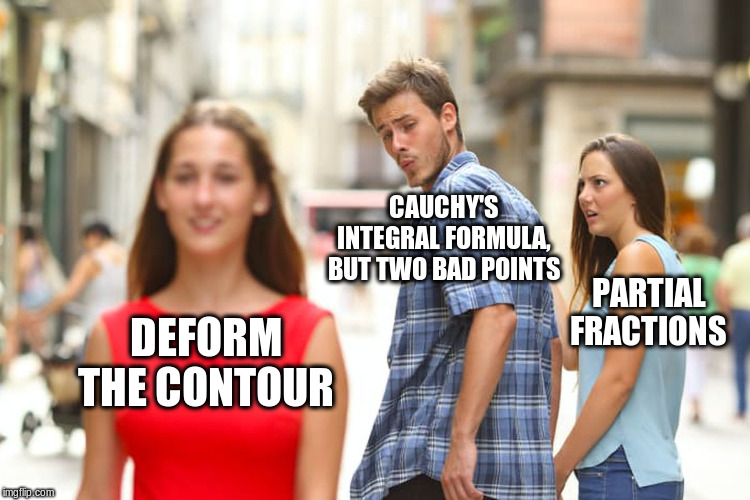
\includegraphics[width=\textwidth,height=0.8\textheight,keepaspectratio]{DistractedCauchy.jpg}

Actually, he's staring straight past the woman in the red dress and checking out the man labelled "Residue Theorem".
\end{frame}

\end{document}